\documentclass[aspectratio=169,10pt]{beamer}
\usepackage{amsmath,amssymb}
\usepackage{booktabs}
\usepackage{array}
\usepackage{tikz}
\usepackage{quantikz}
\usepackage{pgfplots}
\pgfplotsset{compat=1.18}
\usetikzlibrary{positioning,arrows.meta,fit,calc}

% -- look ----------------------------------------------------------------
\definecolor{cblue}{HTML}{2A78D6}
\definecolor{corange}{HTML}{EB6834}
\definecolor{caqua}{HTML}{1BAF7A}
\definecolor{cgray}{HTML}{8A8F98}
\definecolor{cpurple}{HTML}{8E5CC9}
\definecolor{cink}{HTML}{1F1F1E}
\setbeamertemplate{navigation symbols}{}
\setbeamertemplate{footline}{\hfill\scriptsize\color{cgray}\insertframenumber\hspace{0.6em}\vspace{0.4em}}
\setbeamercolor{frametitle}{fg=cblue}
\setbeamercolor{structure}{fg=cblue}
\setbeamercolor{normal text}{fg=cink}
\setbeamerfont{frametitle}{series=\bfseries, size=\large}
\setbeamertemplate{itemize items}{\color{cblue}\textbullet}
\setbeamertemplate{blocks}[rounded]
\setbeamercolor{block title}{bg=cblue!12, fg=cblue}
\setbeamercolor{block body}{bg=cblue!4}
\pgfplotsset{
  every axis/.append style={font=\scriptsize, grid=major, grid style={gray!20},
    legend style={font=\tiny, draw=none, fill=white, fill opacity=0.85, text opacity=1},
    tick label style={font=\tiny}, label style={font=\scriptsize}, title style={font=\scriptsize}},
}
\tikzset{box/.style={draw=cblue, fill=cblue!6, rounded corners=2pt, font=\scriptsize,
  align=center, inner sep=3pt, minimum height=0.8cm},
  val/.style={font=\scriptsize\itshape, text=cgray},
  arr/.style={-{Stealth[length=4pt]}, cgray, thick}}
\newcommand{\key}{\operatorname{key}}
\newcommand{\can}{\operatorname{can}}
\newcolumntype{L}[1]{>{\raggedright\arraybackslash}p{#1}}
\pdfstringdefDisableCommands{\def\translate#1{#1}}

\title{Isogenies on Oasis}
\subtitle{Qiskit Fall Fest 2026, Track 1}
\author{Three Qiskiteers}
\date{November 2026}

\begin{document}

\begin{frame}
\titlepage
\end{frame}

% =========================================================================
\begin{frame}{The campus}
\begin{columns}[T]
\begin{column}{0.36\textwidth}
\centering
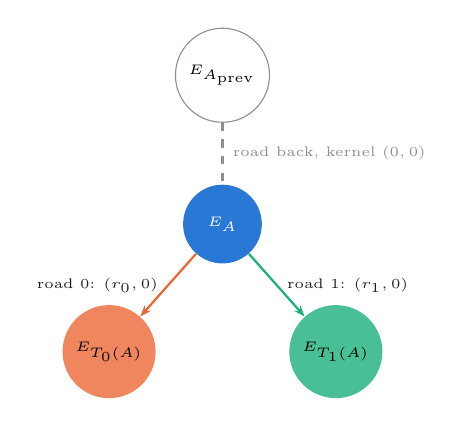
\begin{tikzpicture}[font=\tiny, scale=0.9]
\node[circle, fill=cblue, text=white, minimum size=1.0cm] (A) at (0,0) {$E_A$};
\node[circle, draw=cgray, minimum size=0.9cm] (P) at (0,2.1) {$E_{A_{\rm prev}}$};
\node[circle, fill=corange!80, minimum size=0.9cm] (B0) at (-1.6,-1.8) {$E_{T_0(A)}$};
\node[circle, fill=caqua!80, minimum size=0.9cm] (B1) at (1.6,-1.8) {$E_{T_1(A)}$};
\draw[dashed, cgray, thick] (P) -- node[right] {road back, kernel $(0,0)$} (A);
\draw[arr, corange] (A) -- node[left, text=cink] {road 0: $(r_0,0)$} (B0);
\draw[arr, caqua] (A) -- node[right, text=cink] {road 1: $(r_1,0)$} (B1);
\end{tikzpicture}
\end{column}
\begin{column}{0.62\textwidth}
\begin{itemize}\small
\item A spot is a curve $E_A:\ y^2=x^3+Ax^2+x$, with $A\in\mathbb F=\mathbb F_p(i)$, $p\equiv3\pmod 4$.
\item A road is a 2-isogeny. Its kernel is one 2-torsion point $(r,0)$:
\[ r_{0,1}=\frac{-A\pm\sqrt{A^2-4}}{2},\quad \text{sorted by } \key(u+vi)=u+pv. \]
\item Bit $b$ takes the road through $r_b$:
\[ T_b(A)=\can(2-4r_b^2),\quad \can(z)=\text{the smaller key of } \pm z. \]
\item A password is a route $x=b_1\cdots b_L$. It ends at
\[ H(x)=j(E_{A_L})=\frac{256(A_L^2-3)^3}{A_L^2-4}. \]
\item Small campus: $p=1019$, $A_0=977+297i$, $L=12$, $j^*=797+921i$.
\end{itemize}
\end{column}
\end{columns}
\end{frame}

% =========================================================================
\begin{frame}{Constraints}
\begin{columns}[T]
\begin{column}{0.5\textwidth}
\begin{block}{Search rules}
\begin{itemize}\small
\item The survey walks each road once (at most 2 moves per spot). It does not use $A_0$, $L$ or $j^*$.
\item After the survey: no path counting, no search backwards from ANC, no meet-in-the-middle, no route lists.
\item The only classical work: walk one measured route once, to check it.
\item The test ``are we at ANC?'' reads the spot inside the circuit. It is not built from $H$.
\item If no route gets to ANC, the code says so.
\end{itemize}
\end{block}
\end{column}
\begin{column}{0.46\textwidth}
\begin{block}{Build rules}
\begin{itemize}\small
\item All circuits are built and run in Qiskit.
\item Resources are given after transpiling to a stated basis: queries, qubits, two-qubit gates, depth. Part III also gives the Toffoli and $T$ counts.
\item One command reproduces every result. It takes $p$, $A_0$, $L$, $j^*$.
\item One query is one use of the one-step circuit.
\end{itemize}
\end{block}
\end{column}
\end{columns}
\end{frame}

% =========================================================================
\section{Part I}
\begin{frame}{Part I: the circuit}
\centering
\begin{quantikz}[ampersand replacement=\&, row sep={0.62cm,between origins}, column sep=0.32cm, font=\scriptsize]
\lstick{route $\ket{0}^{\otimes 12}$} \& \qwbundle{12} \& \gate{H^{\otimes12}} \& \gate[3]{W}\gategroup[3,steps=4,style={dashed, rounded corners, draw=cblue}]{Grover iteration, repeated $r$ times} \& \& \gate[3]{W^\dagger} \& \gate{D} \& \meter{} \\
\lstick{merge $\ket{0}^{\otimes 2}$} \& \qwbundle{2} \& \& \& \& \& \& \\
\lstick{spot $\ket{\mathrm{code}(A_0)}$} \& \qwbundle{8} \& \& \& \gate{(-1)^{[A=\mathrm{ANC}]}} \& \& \&
\end{quantikz}

\vspace{0.3em}
\begin{columns}[T]
\begin{column}{0.36\textwidth}
\centering
\begin{quantikz}[ampersand replacement=\&, row sep={0.55cm,between origins}, column sep=0.3cm, font=\scriptsize]
\lstick{$b_t$} \& \gate[3]{\mathrm{Step}} \& \\
\lstick{merge} \& \& \\
\lstick{spot} \& \&
\end{quantikz}\\[2pt]
{\scriptsize $W=\mathrm{Step}_{12}\cdots\mathrm{Step}_1$, step $t$ reads bit $b_t$}
\end{column}
\begin{column}{0.6\textwidth}
\begin{itemize}\small
\item Survey: 255 spots, 510 roads. Each spot gets an 8-bit code.
\item Two merge qubits make the step one-to-one, so it is a permutation. It uses 17 single-target gates (De Vos--Van Rentergem).
\item Oracle $=W$, phase on the ANC codes, $W^\dagger$: 24 queries.
\item 22 qubits. In $\{cx,rz,sx,x\}$: one step 13{,}395 CX, depth 42{,}173.
\end{itemize}
\end{column}
\end{columns}
\end{frame}

% =========================================================================
\begin{frame}{Part I: counting the routes}
\begin{columns}[c]
\begin{column}{0.52\textwidth}
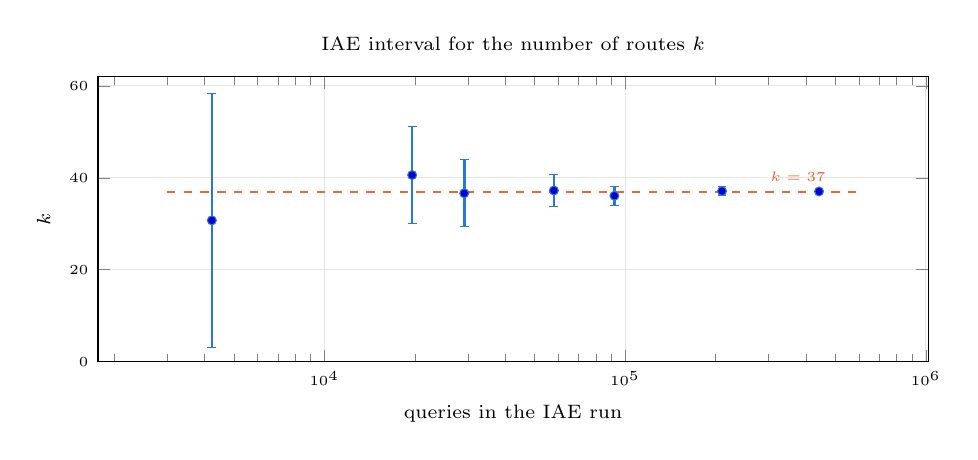
\begin{tikzpicture}
\begin{axis}[width=\linewidth, height=5.2cm, xmode=log,
  xlabel={queries in the IAE run}, ylabel={$k$},
  title={IAE interval for the number of routes $k$}, ymin=0, ymax=62]
\addplot+[cblue, only marks, mark=*, mark size=1.6pt,
  error bars/.cd, y dir=both, y explicit, error bar style={cblue, line width=0.9pt}]
  coordinates {(4224,30.738) +- (0,27.669) (19584,40.603) +- (0,10.582)
  (29184,36.640) +- (0,7.294) (57984,37.242) +- (0,3.474)
  (92160,36.100) +- (0,2.071) (210048,37.105) +- (0,0.914)
  (441600,37.038) +- (0,0.426)};
\addplot[corange, dashed, thick, domain=3000:600000] {37};
\node[corange, font=\tiny, anchor=south east] at (axis cs:500000,37) {$k=37$};
\end{axis}
\end{tikzpicture}
\end{column}
\begin{column}{0.46\textwidth}
\begin{itemize}\small
\item \textbf{IAE} (Iterative Amplitude Estimation): it estimates $a=k/N$ from circuits $Q^m A\ket0$ with Grover powers $Q^m$. It needs no QFT. Each round makes the confidence interval smaller (Appendix A1).
\item We stop when the interval for $k=aN$ holds one integer.
\item Result: $k=37$ at confidence $\ge0.99$.
\item $k=0$ gives an interval at $0$. The code then reports ``no route''.
\end{itemize}
\end{column}
\end{columns}
\end{frame}

% =========================================================================
\begin{frame}{Part I: finding every route}
\begin{columns}[c]
\begin{column}{0.48\textwidth}
\begin{itemize}\small
\item Grover with $r=8$ iterations per run, 137 runs. Each measured route is checked once by one classical walk (1 run rejected).
\item All 37 routes are found. They end at 3 spots:
\end{itemize}
\centering\small
\begin{tabular}{ccc}
\toprule
$A_{12}$ & routes & $j$ \\
\midrule
$3+10i$ & 14 & $797+921i$\\
$933+205i$ & 9 & $797+921i$\\
$561+411i$ & 14 & $797+921i$\\
\bottomrule
\end{tabular}

\vspace{0.4em}
\begin{itemize}\small
\item The 0.99-confidence count costs most of the queries. The scale is $\sqrt{Nk}$ for all routes.
\end{itemize}
\end{column}
\begin{column}{0.5\textwidth}
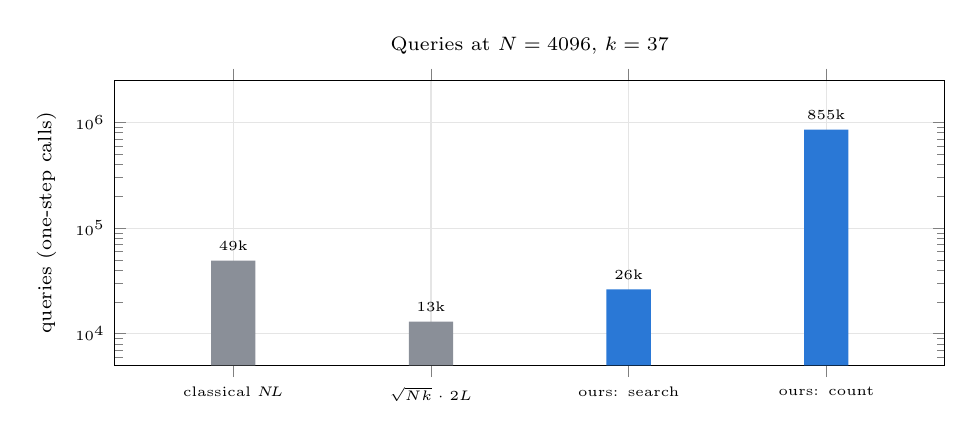
\begin{tikzpicture}
\begin{axis}[width=\linewidth, height=5.2cm, ybar, bar width=16pt,
  ymode=log, log origin=infty, ymin=5000, ymax=2.5e6,
  xtick={1,2,3,4}, xmin=0.4, xmax=4.6,
  xticklabels={classical $N\!L$, $\sqrt{Nk}\cdot2L$, ours: search, ours: count},
  x tick label style={font=\tiny, align=center, text width=1.5cm},
  ylabel={queries (one-step calls)}, title={Queries at $N=4096$, $k=37$},
  nodes near coords, nodes near coords style={font=\tiny},
  point meta=explicit symbolic]
\addplot[fill=cgray, draw=none, bar shift=0pt] coordinates {(1,49152) [49k] (2,13013) [13k]};
\addplot[fill=cblue, draw=none, bar shift=0pt] coordinates {(3,26304) [26k] (4,854784) [855k]};
\end{axis}
\end{tikzpicture}
\end{column}
\end{columns}
\end{frame}

% =========================================================================
\section{Part II}
\begin{frame}{Part II: the target}
\begin{columns}[c]
\begin{column}{0.5\textwidth}
\centering
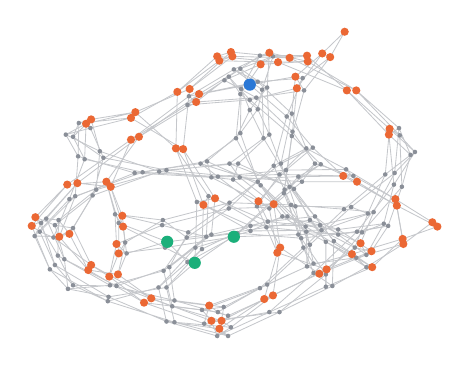
\begin{tikzpicture}[scale=0.92]
% campus p = 1019: 255 spots, 506 roads (generated by a layout script)
\coordinate (v0) at (4.32,4.20);
\coordinate (v1) at (4.12,3.85);
\coordinate (v2) at (3.76,3.39);
\coordinate (v3) at (3.74,3.56);
\coordinate (v4) at (3.10,3.29);
\coordinate (v5) at (3.59,2.76);
\coordinate (v6) at (3.12,3.51);
\coordinate (v7) at (3.52,3.03);
\coordinate (v8) at (2.27,3.23);
\coordinate (v9) at (2.66,3.53);
\coordinate (v10) at (3.99,2.37);
\coordinate (v11) at (3.48,1.97);
\coordinate (v12) at (2.31,3.34);
\coordinate (v13) at (2.79,3.68);
\coordinate (v14) at (3.88,2.60);
\coordinate (v15) at (3.34,2.35);
\coordinate (v16) at (2.17,3.31);
\coordinate (v17) at (1.48,2.75);
\coordinate (v18) at (3.16,3.75);
\coordinate (v19) at (2.89,3.41);
\coordinate (v20) at (3.68,2.20);
\coordinate (v21) at (4.49,2.13);
\coordinate (v22) at (2.79,1.37);
\coordinate (v23) at (3.72,1.35);
\coordinate (v24) at (2.15,3.19);
\coordinate (v25) at (3.28,3.91);
\coordinate (v26) at (3.18,3.40);
\coordinate (v27) at (3.51,2.29);
\coordinate (v28) at (4.30,2.21);
\coordinate (v29) at (2.72,1.76);
\coordinate (v30) at (3.58,1.81);
\coordinate (v31) at (3.01,3.47);
\coordinate (v32) at (0.63,2.11);
\coordinate (v33) at (1.03,2.13);
\coordinate (v34) at (3.81,3.79);
\coordinate (v35) at (3.33,3.86);
\coordinate (v36) at (3.01,3.12);
\coordinate (v37) at (2.88,2.80);
\coordinate (v38) at (3.34,1.82);
\coordinate (v39) at (2.78,2.16);
\coordinate (v40) at (5.04,1.80);
\coordinate (v41) at (4.34,2.30);
\coordinate (v42) at (1.84,1.22);
\coordinate (v43) at (2.15,1.02);
\coordinate (v44) at (4.06,0.85);
\coordinate (v45) at (4.49,1.44);
\coordinate (v46) at (3.01,3.26);
\coordinate (v47) at (3.15,3.87);
\coordinate (v48) at (3.12,3.13);
\coordinate (v49) at (3.20,2.73);
\coordinate (v50) at (3.13,1.86);
\coordinate (v51) at (2.57,2.20);
\coordinate (v52) at (4.44,2.21);
\coordinate (v53) at (1.80,1.53);
\coordinate (v54) at (2.14,1.36);
\coordinate (v55) at (3.84,1.26);
\coordinate (v56) at (4.31,1.75);
\coordinate (v57) at (3.64,3.58);
\coordinate (v58) at (0.13,1.56);
\coordinate (v59) at (0.20,1.62);
\coordinate (v60) at (1.20,1.56);
\coordinate (v61) at (1.15,1.68);
\coordinate (v62) at (4.48,3.39);
\coordinate (v63) at (3.40,3.78);
\coordinate (v64) at (2.88,3.69);
\coordinate (v65) at (3.25,3.43);
\coordinate (v66) at (2.42,2.41);
\coordinate (v67) at (3.12,2.13);
\coordinate (v68) at (3.43,1.22);
\coordinate (v69) at (3.11,1.79);
\coordinate (v70) at (1.76,2.27);
\coordinate (v71) at (2.85,2.38);
\coordinate (v72) at (5.60,1.51);
\coordinate (v73) at (5.13,1.27);
\coordinate (v74) at (3.79,2.59);
\coordinate (v75) at (1.20,1.14);
\coordinate (v76) at (1.26,1.51);
\coordinate (v77) at (2.35,1.20);
\coordinate (v78) at (1.75,0.67);
\coordinate (v79) at (3.42,0.33);
\coordinate (v80) at (4.06,0.68);
\coordinate (v81) at (5.00,2.09);
\coordinate (v82) at (4.92,1.52);
\coordinate (v83) at (3.66,3.42);
\coordinate (v84) at (2.72,3.58);
\coordinate (v85) at (2.88,3.34);
\coordinate (v86) at (2.73,2.38);
\coordinate (v87) at (3.62,2.03);
\coordinate (v88) at (3.28,1.76);
\coordinate (v89) at (1.53,2.26);
\coordinate (v90) at (2.33,2.38);
\coordinate (v91) at (3.91,2.38);
\coordinate (v92) at (1.17,1.27);
\coordinate (v93) at (1.25,1.66);
\coordinate (v94) at (2.48,1.40);
\coordinate (v95) at (1.82,0.90);
\coordinate (v96) at (3.25,0.71);
\coordinate (v97) at (3.80,0.96);
\coordinate (v98) at (4.88,2.23);
\coordinate (v99) at (4.72,1.71);
\coordinate (v100) at (4.01,3.90);
\coordinate (v101) at (0.04,1.38);
\coordinate (v102) at (0.32,0.98);
\coordinate (v103) at (0.37,1.60);
\coordinate (v104) at (0.45,1.06);
\coordinate (v105) at (1.87,1.30);
\coordinate (v106) at (1.81,1.60);
\coordinate (v107) at (5.08,2.77);
\coordinate (v108) at (5.07,2.87);
\coordinate (v109) at (2.59,3.80);
\coordinate (v110) at (2.56,3.86);
\coordinate (v111) at (2.48,2.19);
\coordinate (v112) at (3.78,1.51);
\coordinate (v113) at (3.46,1.65);
\coordinate (v114) at (3.97,0.86);
\coordinate (v115) at (3.33,0.56);
\coordinate (v116) at (3.42,2.23);
\coordinate (v117) at (0.94,2.55);
\coordinate (v118) at (0.84,1.94);
\coordinate (v119) at (3.28,2.78);
\coordinate (v120) at (5.53,1.57);
\coordinate (v121) at (4.48,1.08);
\coordinate (v122) at (4.62,0.95);
\coordinate (v123) at (3.59,3.07);
\coordinate (v124) at (1.29,1.29);
\coordinate (v125) at (1.07,0.82);
\coordinate (v126) at (1.09,2.06);
\coordinate (v127) at (3.02,1.52);
\coordinate (v128) at (2.37,1.81);
\coordinate (v129) at (1.86,0.20);
\coordinate (v130) at (1.05,0.48);
\coordinate (v131) at (2.48,0.21);
\coordinate (v132) at (2.71,0.00);
\coordinate (v133) at (4.06,1.30);
\coordinate (v134) at (4.70,0.95);
\coordinate (v135) at (5.29,2.54);
\coordinate (v136) at (4.93,2.78);
\coordinate (v137) at (4.69,1.17);
\coordinate (v138) at (4.23,1.40);
\coordinate (v139) at (2.87,2.19);
\coordinate (v140) at (4.17,1.31);
\coordinate (v141) at (3.84,1.60);
\coordinate (v142) at (3.73,2.13);
\coordinate (v143) at (0.73,2.44);
\coordinate (v144) at (0.60,1.93);
\coordinate (v145) at (2.82,2.73);
\coordinate (v146) at (3.60,2.82);
\coordinate (v147) at (1.31,1.14);
\coordinate (v148) at (3.26,1.58);
\coordinate (v149) at (2.53,1.90);
\coordinate (v150) at (1.94,0.41);
\coordinate (v151) at (1.08,0.70);
\coordinate (v152) at (2.45,0.42);
\coordinate (v153) at (2.65,0.40);
\coordinate (v154) at (3.79,1.44);
\coordinate (v155) at (4.42,1.13);
\coordinate (v156) at (5.23,2.50);
\coordinate (v157) at (4.94,2.86);
\coordinate (v158) at (4.54,1.28);
\coordinate (v159) at (4.00,1.46);
\coordinate (v160) at (0.52,1.89);
\coordinate (v161) at (0.38,1.37);
\coordinate (v162) at (1.06,0.54);
\coordinate (v163) at (0.57,0.70);
\coordinate (v164) at (0.89,2.02);
\coordinate (v165) at (0.52,1.41);
\coordinate (v166) at (1.17,0.69);
\coordinate (v167) at (0.50,0.65);
\coordinate (v168) at (2.84,1.42);
\coordinate (v169) at (2.73,1.84);
\coordinate (v170) at (5.11,2.06);
\coordinate (v171) at (5.01,2.25);
\coordinate (v172) at (2.77,3.86);
\coordinate (v173) at (2.01,3.37);
\coordinate (v174) at (2.75,3.92);
\coordinate (v175) at (3.89,1.00);
\coordinate (v176) at (3.02,1.45);
\coordinate (v177) at (3.98,1.53);
\coordinate (v178) at (4.46,1.22);
\coordinate (v179) at (4.62,1.12);
\coordinate (v180) at (2.75,0.12);
\coordinate (v181) at (2.71,0.28);
\coordinate (v182) at (0.82,2.99);
\coordinate (v183) at (0.47,2.78);
\coordinate (v184) at (0.32,1.53);
\coordinate (v185) at (5.02,1.89);
\coordinate (v186) at (4.15,0.69);
\coordinate (v187) at (0.82,0.98);
\coordinate (v188) at (1.55,0.46);
\coordinate (v189) at (1.37,2.71);
\coordinate (v190) at (3.53,1.65);
\coordinate (v191) at (2.44,1.93);
\coordinate (v192) at (2.09,2.58);
\coordinate (v193) at (2.56,0.00);
\coordinate (v194) at (2.59,0.10);
\coordinate (v195) at (0.25,0.92);
\coordinate (v196) at (1.65,0.52);
\coordinate (v197) at (2.35,0.36);
\coordinate (v198) at (1.97,0.19);
\coordinate (v199) at (3.56,2.06);
\coordinate (v200) at (5.12,1.34);
\coordinate (v201) at (4.35,3.39);
\coordinate (v202) at (4.07,0.92);
\coordinate (v203) at (3.91,1.65);
\coordinate (v204) at (3.24,1.50);
\coordinate (v205) at (4.23,1.47);
\coordinate (v206) at (0.75,2.93);
\coordinate (v207) at (0.57,2.75);
\coordinate (v208) at (0.11,1.44);
\coordinate (v209) at (2.28,1.85);
\coordinate (v210) at (2.57,0.33);
\coordinate (v211) at (2.62,0.21);
\coordinate (v212) at (0.36,1.11);
\coordinate (v213) at (2.38,0.17);
\coordinate (v214) at (1.97,0.49);
\coordinate (v215) at (3.16,2.08);
\coordinate (v216) at (1.42,2.25);
\coordinate (v217) at (0.57,1.49);
\coordinate (v218) at (0.78,0.91);
\coordinate (v219) at (1.86,0.67);
\coordinate (v220) at (1.86,2.29);
\coordinate (v221) at (0.30,1.36);
\coordinate (v222) at (1.90,0.95);
\coordinate (v223) at (3.49,2.02);
\coordinate (v224) at (3.44,2.38);
\coordinate (v225) at (4.56,1.43);
\coordinate (v226) at (4.41,1.78);
\coordinate (v227) at (3.56,3.84);
\coordinate (v228) at (1.99,2.59);
\coordinate (v229) at (1.37,3.01);
\coordinate (v230) at (3.75,1.22);
\coordinate (v231) at (2.26,1.22);
\coordinate (v232) at (4.64,1.69);
\coordinate (v233) at (4.86,1.55);
\coordinate (v234) at (1.43,3.09);
\coordinate (v235) at (0.65,2.94);
\coordinate (v236) at (0.64,2.48);
\coordinate (v237) at (0.05,1.64);
\coordinate (v238) at (3.89,0.87);
\coordinate (v239) at (2.41,1.37);
\coordinate (v240) at (2.18,3.41);
\coordinate (v241) at (3.28,0.33);
\coordinate (v242) at (3.21,0.51);
\coordinate (v243) at (0.00,1.52);
\coordinate (v244) at (1.19,0.85);
\coordinate (v245) at (3.15,0.66);
\coordinate (v246) at (3.80,3.87);
\coordinate (v247) at (3.39,1.15);
\coordinate (v248) at (0.81,2.87);
\coordinate (v249) at (0.99,2.46);
\coordinate (v250) at (2.25,1.01);
\coordinate (v251) at (2.16,1.43);
\coordinate (v252) at (3.68,1.40);
\coordinate (v253) at (3.64,1.79);
\coordinate (v254) at (0.49,2.09);
\draw[cgray!50, line width=0.3pt] (v0)--(v1) (v0)--(v100) (v1)--(v2) (v1)--(v3) (v1)--(v100) (v2)--(v4) (v2)--(v5) (v2)--(v57) (v3)--(v6) (v3)--(v7) (v3)--(v83) (v4)--(v8) (v4)--(v9) (v4)--(v146) (v5)--(v10) (v5)--(v11) (v5)--(v46) (v6)--(v12) (v6)--(v13) (v6)--(v123) (v7)--(v14) (v7)--(v15) (v7)--(v31) (v8)--(v16) (v8)--(v17) (v8)--(v84) (v9)--(v18) (v9)--(v19) (v9)--(v24) (v10)--(v20) (v10)--(v21) (v10)--(v223) (v11)--(v22) (v11)--(v23) (v11)--(v91) (v12)--(v17) (v12)--(v24) (v12)--(v64) (v13)--(v16) (v13)--(v25) (v13)--(v26) (v14)--(v27) (v14)--(v28) (v14)--(v224) (v15)--(v29) (v15)--(v30) (v15)--(v74) (v16)--(v31) (v16)--(v189) (v17)--(v32) (v17)--(v33) (v18)--(v34) (v18)--(v35) (v18)--(v85) (v19)--(v36) (v19)--(v37) (v19)--(v47) (v20)--(v38) (v20)--(v39) (v20)--(v52);
\draw[cgray!50, line width=0.3pt] (v21)--(v40) (v21)--(v41) (v21)--(v142) (v22)--(v42) (v22)--(v43) (v22)--(v252) (v23)--(v44) (v23)--(v45) (v23)--(v168) (v24)--(v46) (v24)--(v189) (v25)--(v34) (v25)--(v47) (v25)--(v65) (v26)--(v35) (v26)--(v48) (v26)--(v49) (v27)--(v41) (v27)--(v50) (v27)--(v51) (v28)--(v40) (v28)--(v52) (v28)--(v116) (v29)--(v53) (v29)--(v54) (v29)--(v253) (v30)--(v55) (v30)--(v56) (v30)--(v169) (v31)--(v57) (v31)--(v64) (v32)--(v58) (v32)--(v59) (v32)--(v126) (v33)--(v60) (v33)--(v61) (v33)--(v254) (v34)--(v62) (v34)--(v63) (v35)--(v64) (v35)--(v246) (v36)--(v49) (v36)--(v65) (v36)--(v145) (v37)--(v48) (v37)--(v66) (v37)--(v67) (v38)--(v68) (v38)--(v69) (v38)--(v139) (v39)--(v70) (v39)--(v71) (v39)--(v88) (v40)--(v72) (v40)--(v73) (v41)--(v74) (v41)--(v185) (v42)--(v75) (v42)--(v76) (v42)--(v250);
\draw[cgray!50, line width=0.3pt] (v43)--(v77) (v43)--(v78) (v43)--(v105) (v44)--(v79) (v44)--(v80) (v44)--(v225) (v45)--(v81) (v45)--(v82) (v45)--(v238) (v46)--(v83) (v46)--(v84) (v47)--(v84) (v47)--(v246) (v48)--(v85) (v48)--(v119) (v49)--(v86) (v49)--(v87) (v50)--(v68) (v50)--(v88) (v50)--(v111) (v51)--(v69) (v51)--(v89) (v51)--(v90) (v52)--(v91) (v52)--(v185) (v53)--(v92) (v53)--(v93) (v53)--(v251) (v54)--(v94) (v54)--(v95) (v54)--(v106) (v55)--(v96) (v55)--(v97) (v55)--(v226) (v56)--(v98) (v56)--(v99) (v56)--(v230) (v57)--(v100) (v57)--(v123) (v58)--(v101) (v58)--(v102) (v58)--(v237) (v59)--(v103) (v59)--(v104) (v59)--(v243) (v60)--(v75) (v60)--(v93) (v60)--(v105) (v61)--(v76) (v61)--(v92) (v61)--(v106) (v62)--(v107) (v62)--(v108) (v62)--(v227) (v63)--(v109) (v63)--(v110) (v63)--(v201) (v64)--(v65) (v65)--(v119) (v66)--(v89);
\draw[cgray!50, line width=0.3pt] (v66)--(v111) (v66)--(v215) (v67)--(v90) (v67)--(v112) (v67)--(v113) (v68)--(v114) (v68)--(v115) (v69)--(v116) (v69)--(v247) (v70)--(v86) (v70)--(v117) (v70)--(v118) (v71)--(v87) (v71)--(v119) (v71)--(v220) (v72)--(v120) (v72)--(v200) (v73)--(v120) (v73)--(v121) (v73)--(v122) (v74)--(v116) (v74)--(v123) (v75)--(v124) (v75)--(v125) (v76)--(v126) (v76)--(v147) (v77)--(v127) (v77)--(v128) (v77)--(v219) (v78)--(v129) (v78)--(v130) (v78)--(v231) (v79)--(v131) (v79)--(v132) (v79)--(v186) (v80)--(v133) (v80)--(v134) (v80)--(v241) (v81)--(v135) (v81)--(v136) (v81)--(v233) (v82)--(v137) (v82)--(v138) (v82)--(v170) (v83)--(v100) (v83)--(v146) (v84)--(v85) (v85)--(v145) (v86)--(v139) (v86)--(v199) (v87)--(v140) (v87)--(v141) (v88)--(v142) (v88)--(v247) (v89)--(v143) (v89)--(v144) (v90)--(v145) (v90)--(v216) (v91)--(v142) (v91)--(v146);
\draw[cgray!50, line width=0.3pt] (v92)--(v125) (v92)--(v147) (v93)--(v124) (v93)--(v126) (v94)--(v148) (v94)--(v149) (v94)--(v222) (v95)--(v150) (v95)--(v151) (v95)--(v239) (v96)--(v152) (v96)--(v153) (v96)--(v175) (v97)--(v154) (v97)--(v155) (v97)--(v245) (v98)--(v156) (v98)--(v157) (v98)--(v232) (v99)--(v158) (v99)--(v159) (v99)--(v171) (v101)--(v160) (v101)--(v161) (v101)--(v195) (v102)--(v162) (v102)--(v163) (v102)--(v208) (v103)--(v164) (v103)--(v165) (v103)--(v212) (v104)--(v166) (v104)--(v167) (v104)--(v184) (v105)--(v147) (v105)--(v168) (v106)--(v124) (v106)--(v169) (v107)--(v135) (v107)--(v157) (v107)--(v170) (v108)--(v136) (v108)--(v156) (v108)--(v171) (v109)--(v172) (v109)--(v173) (v110)--(v173) (v110)--(v174) (v111)--(v116) (v111)--(v216) (v112)--(v155) (v112)--(v175) (v112)--(v190) (v113)--(v154) (v113)--(v176) (v113)--(v177) (v114)--(v178) (v114)--(v179) (v114)--(v242) (v115)--(v180);
\draw[cgray!50, line width=0.3pt] (v115)--(v181) (v115)--(v202) (v117)--(v164) (v117)--(v182) (v117)--(v183) (v118)--(v165) (v118)--(v184) (v118)--(v249) (v119)--(v199) (v120)--(v185) (v121)--(v134) (v121)--(v154) (v121)--(v175) (v122)--(v133) (v122)--(v155) (v122)--(v186) (v123)--(v224) (v124)--(v244) (v125)--(v187) (v125)--(v188) (v126)--(v189) (v127)--(v177) (v127)--(v190) (v127)--(v209) (v128)--(v176) (v128)--(v191) (v128)--(v192) (v129)--(v162) (v129)--(v193) (v129)--(v194) (v130)--(v163) (v130)--(v195) (v130)--(v198) (v131)--(v193) (v131)--(v196) (v131)--(v197) (v132)--(v194) (v132)--(v198) (v132)--(v213) (v133)--(v141) (v133)--(v199) (v134)--(v140) (v134)--(v200) (v135)--(v157) (v135)--(v171) (v136)--(v156) (v136)--(v201) (v137)--(v178) (v137)--(v202) (v137)--(v205) (v138)--(v179) (v138)--(v203) (v138)--(v204) (v139)--(v142) (v139)--(v220) (v140)--(v186) (v140)--(v203) (v141)--(v204) (v141)--(v205) (v143)--(v160);
\draw[cgray!50, line width=0.3pt] (v143)--(v206) (v143)--(v207) (v144)--(v161) (v144)--(v208) (v144)--(v236) (v145)--(v215) (v146)--(v223) (v147)--(v244) (v148)--(v191) (v148)--(v203) (v148)--(v205) (v149)--(v192) (v149)--(v204) (v149)--(v209) (v150)--(v166) (v150)--(v210) (v150)--(v211) (v151)--(v167) (v151)--(v212) (v151)--(v214) (v152)--(v196) (v152)--(v210) (v152)--(v213) (v153)--(v197) (v153)--(v211) (v153)--(v214) (v154)--(v215) (v155)--(v200) (v156)--(v170) (v157)--(v201) (v158)--(v177) (v158)--(v179) (v158)--(v202) (v159)--(v176) (v159)--(v178) (v159)--(v190) (v160)--(v216) (v160)--(v221) (v161)--(v217) (v161)--(v218) (v162)--(v167) (v162)--(v219) (v163)--(v166) (v163)--(v212) (v164)--(v217) (v164)--(v220) (v165)--(v218) (v165)--(v221) (v166)--(v222) (v167)--(v195) (v168)--(v223) (v168)--(v250) (v169)--(v224) (v169)--(v251) (v170)--(v225) (v171)--(v226) (v172)--(v227) (v172)--(v240) (v173)--(v228) (v173)--(v229);
\draw[cgray!50, line width=0.3pt] (v174)--(v227) (v174)--(v240) (v175)--(v230) (v176)--(v231) (v177)--(v232) (v178)--(v232) (v179)--(v233) (v180)--(v193) (v180)--(v198) (v180)--(v211) (v181)--(v194) (v181)--(v210) (v181)--(v214) (v182)--(v207) (v182)--(v234) (v182)--(v235) (v183)--(v206) (v183)--(v236) (v183)--(v248) (v184)--(v217) (v184)--(v237) (v185)--(v200) (v186)--(v238) (v187)--(v196) (v187)--(v217) (v187)--(v221) (v188)--(v197) (v188)--(v213) (v188)--(v218) (v189)--(v254) (v190)--(v215) (v191)--(v228) (v191)--(v239) (v192)--(v229) (v192)--(v240) (v193)--(v241) (v194)--(v242) (v195)--(v243) (v196)--(v244) (v197)--(v245) (v198)--(v219) (v199)--(v203) (v201)--(v246) (v202)--(v247) (v204)--(v239) (v205)--(v233) (v206)--(v234) (v206)--(v248) (v207)--(v235) (v207)--(v249) (v208)--(v221) (v208)--(v243) (v209)--(v228) (v209)--(v231) (v210)--(v245) (v211)--(v242) (v212)--(v237) (v213)--(v241) (v214)--(v222) (v216)--(v236);
\draw[cgray!50, line width=0.3pt] (v218)--(v244) (v219)--(v250) (v220)--(v249) (v222)--(v251) (v223)--(v252) (v224)--(v253) (v225)--(v233) (v225)--(v252) (v226)--(v232) (v226)--(v253) (v227)--(v246) (v228)--(v234) (v229)--(v235) (v229)--(v248) (v230)--(v245) (v230)--(v253) (v231)--(v250) (v234)--(v240) (v235)--(v236) (v237)--(v254) (v238)--(v241) (v238)--(v252) (v239)--(v251) (v242)--(v247) (v243)--(v254) (v248)--(v249);
\fill[cgray] (v0) circle (0.9pt) (v1) circle (0.9pt) (v2) circle (0.9pt) (v3) circle (0.9pt) (v4) circle (0.9pt) (v5) circle (0.9pt) (v6) circle (0.9pt) (v7) circle (0.9pt) (v8) circle (0.9pt) (v9) circle (0.9pt) (v10) circle (0.9pt) (v11) circle (0.9pt) (v12) circle (0.9pt) (v13) circle (0.9pt) (v14) circle (0.9pt) (v15) circle (0.9pt) (v16) circle (0.9pt) (v17) circle (0.9pt) (v18) circle (0.9pt) (v19) circle (0.9pt) (v20) circle (0.9pt) (v21) circle (0.9pt) (v22) circle (0.9pt) (v23) circle (0.9pt) (v24) circle (0.9pt) (v25) circle (0.9pt) (v26) circle (0.9pt) (v27) circle (0.9pt) (v28) circle (0.9pt) (v29) circle (0.9pt) (v30) circle (0.9pt) (v31) circle (0.9pt) (v32) circle (0.9pt) (v33) circle (0.9pt) (v34) circle (0.9pt) (v35) circle (0.9pt) (v36) circle (0.9pt) (v37) circle (0.9pt) (v38) circle (0.9pt) (v39) circle (0.9pt) (v40) circle (0.9pt) (v41) circle (0.9pt) (v42) circle (0.9pt) (v43) circle (0.9pt) (v44) circle (0.9pt) (v45) circle (0.9pt) (v46) circle (0.9pt) (v47) circle (0.9pt) (v48) circle (0.9pt) (v49) circle (0.9pt) (v50) circle (0.9pt) (v51) circle (0.9pt) (v52) circle (0.9pt) (v53) circle (0.9pt) (v54) circle (0.9pt) (v55) circle (0.9pt) (v56) circle (0.9pt) (v57) circle (0.9pt) (v58) circle (0.9pt) (v59) circle (0.9pt);
\fill[cgray] (v60) circle (0.9pt) (v61) circle (0.9pt) (v62) circle (0.9pt) (v63) circle (0.9pt) (v64) circle (0.9pt) (v65) circle (0.9pt) (v66) circle (0.9pt) (v67) circle (0.9pt) (v68) circle (0.9pt) (v69) circle (0.9pt) (v70) circle (0.9pt) (v71) circle (0.9pt) (v72) circle (0.9pt) (v73) circle (0.9pt) (v74) circle (0.9pt) (v75) circle (0.9pt) (v76) circle (0.9pt) (v77) circle (0.9pt) (v78) circle (0.9pt) (v79) circle (0.9pt) (v80) circle (0.9pt) (v81) circle (0.9pt) (v82) circle (0.9pt) (v83) circle (0.9pt) (v84) circle (0.9pt) (v85) circle (0.9pt) (v86) circle (0.9pt) (v87) circle (0.9pt) (v88) circle (0.9pt) (v89) circle (0.9pt) (v90) circle (0.9pt) (v91) circle (0.9pt) (v92) circle (0.9pt) (v93) circle (0.9pt) (v94) circle (0.9pt) (v95) circle (0.9pt) (v96) circle (0.9pt) (v97) circle (0.9pt) (v98) circle (0.9pt) (v99) circle (0.9pt) (v100) circle (0.9pt) (v101) circle (0.9pt) (v102) circle (0.9pt) (v103) circle (0.9pt) (v104) circle (0.9pt) (v105) circle (0.9pt) (v106) circle (0.9pt) (v107) circle (0.9pt) (v108) circle (0.9pt) (v109) circle (0.9pt) (v110) circle (0.9pt) (v111) circle (0.9pt) (v112) circle (0.9pt) (v113) circle (0.9pt) (v114) circle (0.9pt) (v115) circle (0.9pt) (v116) circle (0.9pt) (v117) circle (0.9pt) (v118) circle (0.9pt) (v119) circle (0.9pt);
\fill[cgray] (v120) circle (0.9pt) (v121) circle (0.9pt) (v122) circle (0.9pt) (v123) circle (0.9pt) (v124) circle (0.9pt) (v125) circle (0.9pt) (v126) circle (0.9pt) (v127) circle (0.9pt) (v128) circle (0.9pt) (v129) circle (0.9pt) (v130) circle (0.9pt) (v131) circle (0.9pt) (v132) circle (0.9pt) (v133) circle (0.9pt) (v134) circle (0.9pt) (v135) circle (0.9pt) (v136) circle (0.9pt) (v137) circle (0.9pt) (v138) circle (0.9pt) (v139) circle (0.9pt) (v140) circle (0.9pt) (v141) circle (0.9pt) (v142) circle (0.9pt) (v143) circle (0.9pt) (v144) circle (0.9pt) (v145) circle (0.9pt) (v146) circle (0.9pt) (v147) circle (0.9pt) (v148) circle (0.9pt) (v149) circle (0.9pt) (v150) circle (0.9pt) (v151) circle (0.9pt) (v152) circle (0.9pt) (v153) circle (0.9pt) (v154) circle (0.9pt) (v155) circle (0.9pt) (v156) circle (0.9pt) (v157) circle (0.9pt) (v158) circle (0.9pt) (v159) circle (0.9pt) (v160) circle (0.9pt) (v161) circle (0.9pt) (v162) circle (0.9pt) (v163) circle (0.9pt) (v164) circle (0.9pt) (v165) circle (0.9pt) (v166) circle (0.9pt) (v167) circle (0.9pt) (v168) circle (0.9pt) (v169) circle (0.9pt) (v170) circle (0.9pt) (v171) circle (0.9pt) (v172) circle (0.9pt) (v173) circle (0.9pt) (v174) circle (0.9pt) (v175) circle (0.9pt) (v176) circle (0.9pt) (v177) circle (0.9pt) (v178) circle (0.9pt) (v179) circle (0.9pt);
\fill[cgray] (v180) circle (0.9pt) (v181) circle (0.9pt) (v182) circle (0.9pt) (v183) circle (0.9pt) (v184) circle (0.9pt) (v185) circle (0.9pt) (v186) circle (0.9pt) (v187) circle (0.9pt) (v188) circle (0.9pt) (v189) circle (0.9pt) (v190) circle (0.9pt) (v191) circle (0.9pt) (v192) circle (0.9pt) (v193) circle (0.9pt) (v194) circle (0.9pt) (v195) circle (0.9pt) (v196) circle (0.9pt) (v197) circle (0.9pt) (v198) circle (0.9pt) (v199) circle (0.9pt) (v200) circle (0.9pt) (v201) circle (0.9pt) (v202) circle (0.9pt) (v203) circle (0.9pt) (v204) circle (0.9pt) (v205) circle (0.9pt) (v206) circle (0.9pt) (v207) circle (0.9pt) (v208) circle (0.9pt) (v209) circle (0.9pt) (v210) circle (0.9pt) (v211) circle (0.9pt) (v212) circle (0.9pt) (v213) circle (0.9pt) (v214) circle (0.9pt) (v215) circle (0.9pt) (v216) circle (0.9pt) (v217) circle (0.9pt) (v218) circle (0.9pt) (v219) circle (0.9pt) (v220) circle (0.9pt) (v221) circle (0.9pt) (v222) circle (0.9pt) (v223) circle (0.9pt) (v224) circle (0.9pt) (v225) circle (0.9pt) (v226) circle (0.9pt) (v227) circle (0.9pt) (v228) circle (0.9pt) (v229) circle (0.9pt) (v230) circle (0.9pt) (v231) circle (0.9pt) (v232) circle (0.9pt) (v233) circle (0.9pt) (v234) circle (0.9pt) (v235) circle (0.9pt) (v236) circle (0.9pt) (v237) circle (0.9pt) (v238) circle (0.9pt) (v239) circle (0.9pt);
\fill[cgray] (v240) circle (0.9pt) (v241) circle (0.9pt) (v242) circle (0.9pt) (v243) circle (0.9pt) (v244) circle (0.9pt) (v245) circle (0.9pt) (v246) circle (0.9pt) (v247) circle (0.9pt) (v248) circle (0.9pt) (v249) circle (0.9pt) (v250) circle (0.9pt) (v251) circle (0.9pt) (v252) circle (0.9pt) (v253) circle (0.9pt) (v254) circle (0.9pt);
\fill[corange] (v0) circle (1.6pt) (v1) circle (1.6pt) (v8) circle (1.6pt) (v12) circle (1.6pt) (v17) circle (1.6pt) (v18) circle (1.6pt) (v21) circle (1.6pt) (v25) circle (1.6pt) (v28) circle (1.6pt) (v32) circle (1.6pt) (v33) circle (1.6pt) (v34) circle (1.6pt) (v38) circle (1.6pt) (v40) circle (1.6pt) (v50) circle (1.6pt) (v57) circle (1.6pt) (v62) circle (1.6pt) (v63) circle (1.6pt) (v68) circle (1.6pt) (v72) circle (1.6pt) (v73) circle (1.6pt) (v75) circle (1.6pt) (v76) circle (1.6pt) (v83) circle (1.6pt) (v92) circle (1.6pt) (v93) circle (1.6pt) (v100) circle (1.6pt) (v109) circle (1.6pt) (v110) circle (1.6pt) (v114) circle (1.6pt) (v115) circle (1.6pt) (v120) circle (1.6pt) (v125) circle (1.6pt) (v126) circle (1.6pt) (v128) circle (1.6pt) (v131) circle (1.6pt) (v134) circle (1.6pt) (v136) circle (1.6pt) (v137) circle (1.6pt) (v149) circle (1.6pt) (v152) circle (1.6pt) (v155) circle (1.6pt) (v157) circle (1.6pt) (v158) circle (1.6pt) (v161) circle (1.6pt) (v165) circle (1.6pt) (v172) circle (1.6pt) (v173) circle (1.6pt) (v174) circle (1.6pt) (v182) circle (1.6pt) (v185) circle (1.6pt) (v187) circle (1.6pt) (v188) circle (1.6pt) (v189) circle (1.6pt) (v192) circle (1.6pt) (v194) circle (1.6pt) (v196) circle (1.6pt) (v200) circle (1.6pt) (v201) circle (1.6pt) (v202) circle (1.6pt);
\fill[corange] (v206) circle (1.6pt) (v211) circle (1.6pt) (v218) circle (1.6pt) (v227) circle (1.6pt) (v228) circle (1.6pt) (v229) circle (1.6pt) (v234) circle (1.6pt) (v237) circle (1.6pt) (v240) circle (1.6pt) (v242) circle (1.6pt) (v243) circle (1.6pt) (v244) circle (1.6pt) (v246) circle (1.6pt) (v247) circle (1.6pt) (v254) circle (1.6pt);
\fill[caqua] (v22) circle (2.4pt) (v105) circle (2.4pt) (v250) circle (2.4pt);
\fill[cblue] (v31) circle (2.4pt);
\end{tikzpicture}\\
{\scriptsize\color{cgray} $p=1019$: 255 spots.
\textcolor{corange}{$\bullet$} on the tower (75),
\textcolor{caqua}{$\bullet$} ANC (3), \textcolor{cblue}{$\bullet$} $A_0$}
\end{column}
\begin{column}{0.48\textwidth}
\begin{itemize}\small
\item Top of the Clock Tower: $T_p=\{E: j(E)\in\mathbb F_p\}$.
\item Deuring--Eichler: $|T_p|=2h(-p)$ or $h(-p)$, where $h$ is a class number.
\item Siegel: $h(-p)=p^{1/2+o(1)}$. All spots: $|V_p|=p/12+O(1)$.
\end{itemize}
\[ \frac{|T_p|}{|V_p|}=p^{-1/2+o(1)} \]
\begin{itemize}\small
\item Small campus: 75 of 255 spots (29\%). At $p\approx2^{256}$: about 1 spot in $2^{125}$.
\end{itemize}
\end{column}
\end{columns}
\end{frame}

% =========================================================================
\begin{frame}{Part II: from spots to routes}
\begin{columns}[c]
\begin{column}{0.5\textwidth}
\begin{itemize}\small
\item A route is a walk without backtracking on a 3-regular Ramanujan graph (Pizer).
\item Lubetzky--Peres: the end of the walk is close to uniform,
\[ d_{\rm TV}\le O\big(\sqrt{p}\,2^{-L/2}L\big). \]
\item With $L=\lceil3\log_2p\rceil$ this is $\widetilde O(p^{-1})$, much less than the target fraction. So
\[ q_L=\Pr_x[f(x)=1]=p^{-1/2+o(1)}. \]
\item Data (right): route fraction $=$ spot fraction, for 40 primes, already with $L=2\lceil\log_2p\rceil$.
\end{itemize}
\end{column}
\begin{column}{0.48\textwidth}
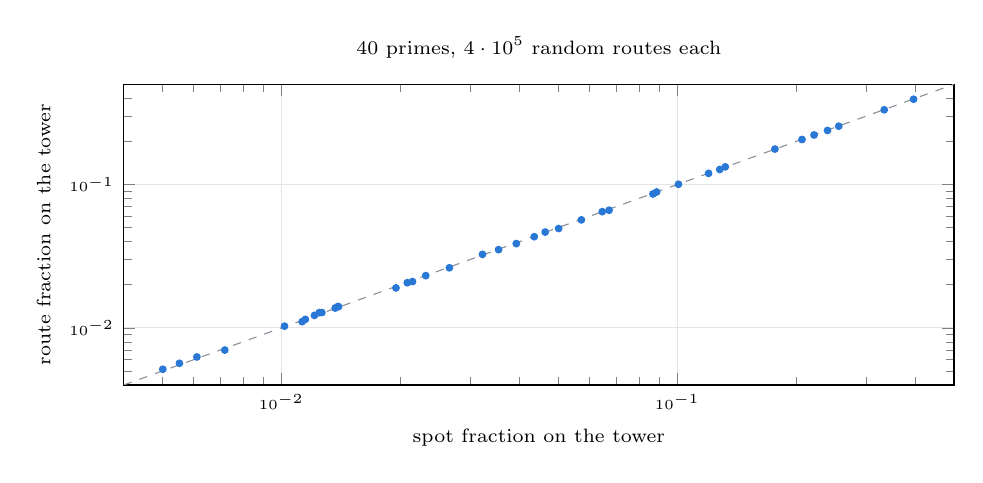
\begin{tikzpicture}
\begin{axis}[width=\linewidth, height=5.4cm, xmode=log, ymode=log,
  xlabel={spot fraction on the tower}, ylabel={route fraction on the tower},
  title={40 primes, $4\cdot10^5$ random routes each}, xmin=4e-3, xmax=0.5, ymin=4e-3, ymax=0.5]
\addplot[cgray, dashed, domain=4e-3:0.5, samples=2] {x};
\addplot[cblue, only marks, mark=*, mark size=1.2pt] coordinates {(0.39535,0.393470) (0.33333,0.332168) (0.20661,0.206083) (0.06729,0.066175) (0.25581,0.255248) (0.17647,0.176725) (0.23967,0.238303) (0.06467,0.064702) (0.08683,0.085947) (0.22167,0.221660) (0.13223,0.132830) (0.12000,0.119650) (0.10073,0.100453) (0.12808,0.127342) (0.02658,0.026270) (0.08870,0.088703) (0.03924,0.038730) (0.02317,0.023152) (0.01948,0.019015) (0.04640,0.046608) (0.05016,0.049340) (0.02145,0.021050) (0.03538,0.035153) (0.04354,0.043280) (0.02081,0.020665) (0.05727,0.056717) (0.01368,0.013760) (0.01019,0.010287) (0.03222,0.032575) (0.01129,0.011060) (0.01150,0.011465) (0.01386,0.014045) (0.00502,0.005150) (0.01266,0.012795) (0.01213,0.012230) (0.01247,0.012778) (0.00553,0.005667) (0.01395,0.014090) (0.00720,0.007010) (0.00612,0.006275)};
\end{axis}
\end{tikzpicture}
\end{column}
\end{columns}
\end{frame}

% =========================================================================
\begin{frame}{Part II: the upper bound}
\centering
\begin{quantikz}[ampersand replacement=\&, row sep={0.62cm,between origins}, column sep=0.32cm, font=\scriptsize]
\lstick{route $x$} \& \qwbundle{L} \& \gate{H^{\otimes L}} \& \gate[3]{W}\gategroup[4,steps=4,style={dashed, rounded corners, draw=cblue}]{oracle $O_f$: $2L$ queries} \& \& \& \gate[3]{W^\dagger} \& \gate{D} \& \meter{}\\
\lstick{$A_0$} \& \qwbundle{2n} \& \& \& \& \& \& \& \\
\lstick{$A_1\ldots A_L$} \& \qwbundle{2nL} \& \& \& \gate[2]{\text{tower test}} \& \& \& \& \\
\lstick{flag $\ket{-}$} \& \& \& \& \& \& \& \&
\end{quantikz}

\vspace{0.4em}
\begin{columns}[T]
\begin{column}{0.5\textwidth}
\begin{itemize}\small
\item $O_f\ket x=(-1)^{f(x)}\ket x$, $f(x)=[\,j(E_{A_L(x)})\in\mathbb F_p\,]$.
\item With $\sin^2\theta=q_L$: after $t$ iterations,
$P(t)=\sin^2((2t+1)\theta)$.
\end{itemize}
\end{column}
\begin{column}{0.48\textwidth}
\begin{itemize}\small
\item $t\approx\frac{\pi}{4\sqrt{q_L}}=p^{1/4+o(1)}$ iterations, each $2L=O(\log p)$ queries.
\item $q_L$ unknown: BBHT, at most $\tfrac94\sqrt{1/q_L}$ on average.
\item Classical random routes: $1/q_L=p^{1/2+o(1)}$.
\end{itemize}
\end{column}
\end{columns}
\end{frame}

% =========================================================================
\begin{frame}{Part II: the lower bound}
\begin{columns}[T]
\begin{column}{0.5\textwidth}
\begin{block}{Black-box model}
\small
Input: an unknown $f:\{0,1\}^L\to\{0,1\}$ with $k$ marked inputs. The only access is the oracle $O_f\ket{x,z}=\ket{x,z\oplus f(x)}$.

\medskip
BBBV, Zalka: every quantum algorithm with constant success needs
\[ \Omega\big(\sqrt{N/k}\big)=\Omega\big(q_L^{-1/2}\big)=\Omega\big(p^{1/4-o(1)}\big) \]
oracle queries. Grover meets this bound.
\end{block}
\end{column}
\begin{column}{0.46\textwidth}
\begin{block}{The real arithmetic}
\small
\begin{itemize}
\item The step is explicit field arithmetic. An algorithm can use this structure, so the black-box bound does not apply.
\item ``A route to the tower exists'' is in NP (Appendix A3). A proof that no polynomial-time quantum algorithm exists would show NP $\not\subseteq$ BQP, and so P $\neq$ NP.
\item No known algorithm beats $p^{1/4}$ under these rules (Appendix A4).
\end{itemize}
\end{block}
\end{column}
\end{columns}
\end{frame}

% =========================================================================
\begin{frame}{Part II: data}
\begin{columns}[c]
\begin{column}{0.6\textwidth}
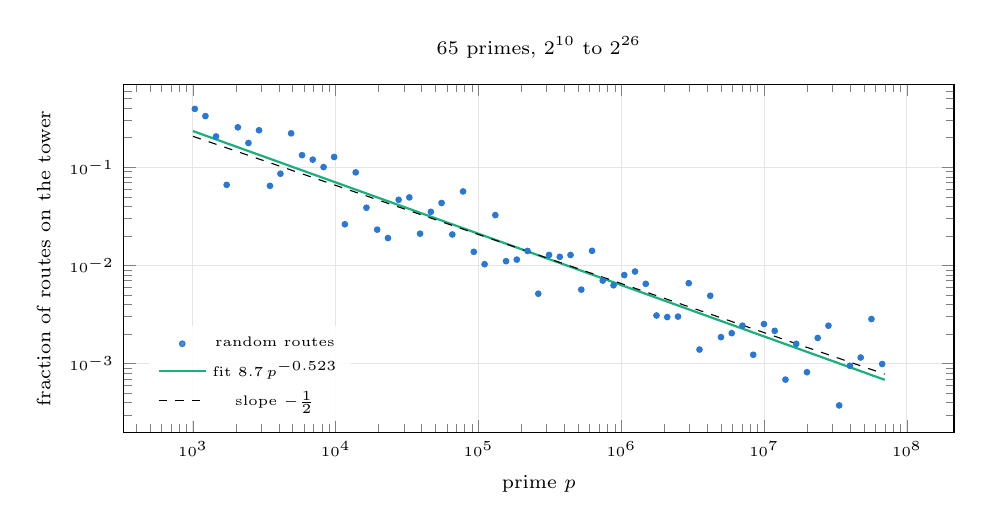
\begin{tikzpicture}
\begin{axis}[width=\linewidth, height=6.0cm, xmode=log, ymode=log,
  xlabel={prime $p$}, ylabel={fraction of routes on the tower},
  title={65 primes, $2^{10}$ to $2^{26}$}, legend pos=south west, ymin=2e-4, ymax=0.7]
\addplot[cblue, only marks, mark=*, mark size=1.0pt] coordinates {
(1031,0.393470) (1223,0.332168) (1451,0.206083) (1723,0.066175) (2063,0.255248) (2447,0.176725) (2903,0.238303) (3463,0.064702) (4099,0.085947) (4871,0.221660) (5807,0.132830) (6899,0.119650) (8219,0.100453) (9743,0.127342) (11587,0.026270) (13799,0.088703) (16411,0.038730) (19507,0.023152) (23203,0.019015) (27583,0.046608) (32771,0.049340) (38971,0.021050) (46351,0.035153) (55127,0.043280) (65539,0.020665) (77951,0.056717) (92683,0.013760) (110251,0.010287) (131111,0.032575) (155887,0.011060) (185371,0.011465) (220447,0.014045) (262147,0.005150) (311747,0.012795) (370759,0.012230) (440903,0.012778) (524347,0.005667) (623531,0.014090) (741467,0.007010) (881779,0.006275) (1048583,0.007975) (1247063,0.008670) (1482919,0.006493) (1763491,0.003090) (2097211,0.002980) (2493979,0.003012) (2965847,0.006598) (3526987,0.001390) (4194319,0.004908) (4987903,0.001860) (5931763,0.002043) (7053971,0.002437) (8388619,0.001230) (9975803,0.002527) (11863343,0.002155) (14107963,0.000687) (16777259,0.001590) (19951627,0.000817) (23726579,0.001825) (28215851,0.002433) (33554467,0.000375) (39903203,0.000950) (47453183,0.001153) (56431751,0.002845) (67108879,0.000990)};
\addlegendentry{random routes}
\addplot[caqua, thick, domain=1000:7e7, samples=2] {8.660*x^(-0.523)};
\addlegendentry{fit $8.7\,p^{-0.523}$}
\addplot[black, dashed, domain=1000:7e7, samples=2] {6.538*x^(-0.5)};
\addlegendentry{slope $-\frac12$}
\end{axis}
\end{tikzpicture}
\end{column}
\begin{column}{0.38\textwidth}
\begin{itemize}\small
\item Fit: $\widehat q\approx8.7\,p^{-\alpha}$,
\[ \widehat\alpha=0.523\pm0.040 \]
(65 primes, 2 standard errors).
\item Exact spot fractions, 40 primes: $\widehat\alpha=0.560\pm0.081$.
\item The scatter comes from the class number $h(-p)$, not from noise: the same primes are high in both columns.
\item Theory: $\alpha=\tfrac12$.
\end{itemize}
\end{column}
\end{columns}
\end{frame}

% =========================================================================
\begin{frame}{Part II: demonstration}
\begin{columns}[c]
\begin{column}{0.5\textwidth}
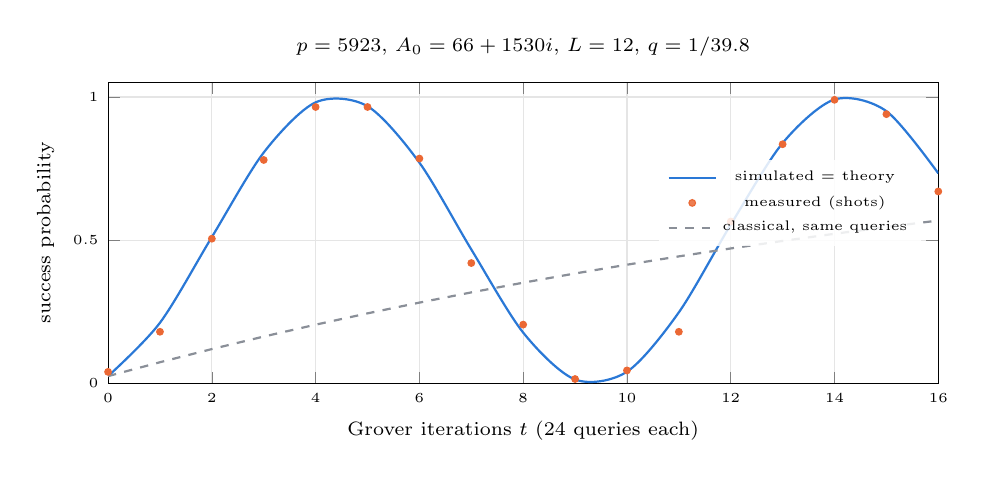
\begin{tikzpicture}
\begin{axis}[width=\linewidth, height=5.4cm, xmin=0, xmax=16, ymin=0, ymax=1.05,
  xlabel={Grover iterations $t$ (24 queries each)}, ylabel={success probability},
  title={$p=5923$, $A_0=66+1530i$, $L=12$, $q=1/39.8$},
  legend style={at={(0.98,0.60)}, anchor=east}]
\addplot[cblue, thick, smooth] coordinates {(0,0.0251) (1,0.2114) (2,0.5108) (3,0.8060)
  (4,0.9812) (5,0.9676) (6,0.7706) (7,0.4675) (8,0.1771) (9,0.0134) (10,0.0405)
  (11,0.2479) (12,0.5541) (13,0.8391) (14,0.9911) (15,0.9505) (16,0.7332)};
\addlegendentry{simulated $=$ theory}
\addplot[corange, only marks, mark=*, mark size=1.2pt] coordinates {(0,0.040) (1,0.180)
  (2,0.505) (3,0.780) (4,0.965) (5,0.965) (6,0.785) (7,0.420) (8,0.205) (9,0.015)
  (10,0.045) (11,0.180) (12,0.565) (13,0.835) (14,0.990) (15,0.940) (16,0.670)};
\addlegendentry{measured (shots)}
\addplot[cgray, thick, dashed] coordinates {(0,0.0251) (1,0.0736) (2,0.1196) (3,0.1633)
  (4,0.2048) (5,0.2443) (6,0.2819) (7,0.3175) (8,0.3514) (9,0.3836) (10,0.4142)
  (11,0.4433) (12,0.4710) (13,0.4972) (14,0.5222) (15,0.5459) (16,0.5685)};
\addlegendentry{classical, same queries}
\end{axis}
\end{tikzpicture}
\end{column}
\begin{column}{0.48\textwidth}
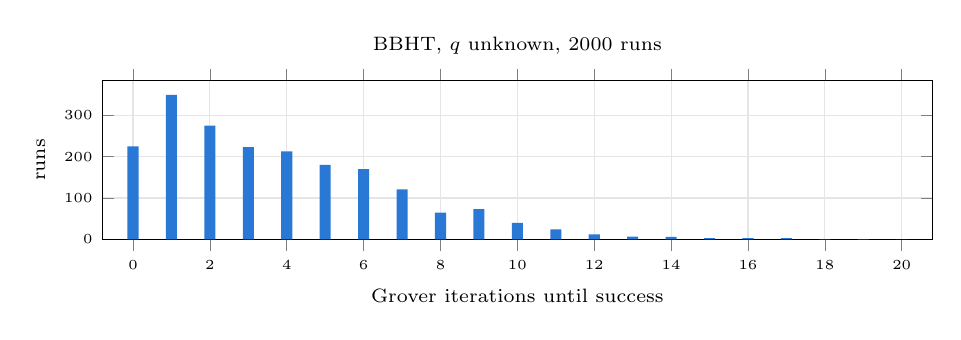
\begin{tikzpicture}
\begin{axis}[width=\linewidth, height=3.6cm, ybar, bar width=4pt, ymin=0,
  xlabel={Grover iterations until success}, ylabel={runs},
  title={BBHT, $q$ unknown, 2000 runs}, xmin=-0.8, xmax=20.8]
\addplot[fill=cblue, draw=none] coordinates {(0,225) (1,349) (2,275) (3,223) (4,213) (5,180) (6,170) (7,121) (8,65) (9,73) (10,40) (11,24) (12,12) (13,7) (14,6) (15,3) (16,3) (17,3) (18,1) (19,1) (20,0)};
\end{axis}
\end{tikzpicture}
\begin{itemize}\small
\item Simulation $=$ theory to 4 decimals. At $t=4$: $0.981$, against $0.205$ classically.
\item BBHT: on average 91 queries and 7.9 checks. Classical: 477 steps.
\item 25 qubits. One iteration in $\{cx,rz,sx,x\}$: $3.40\cdot10^6$ CX, depth $1.11\cdot10^7$.
\end{itemize}
\end{column}
\end{columns}
\end{frame}

% =========================================================================
\section{Part III}
\begin{frame}{Part III: one step from arithmetic}
\centering
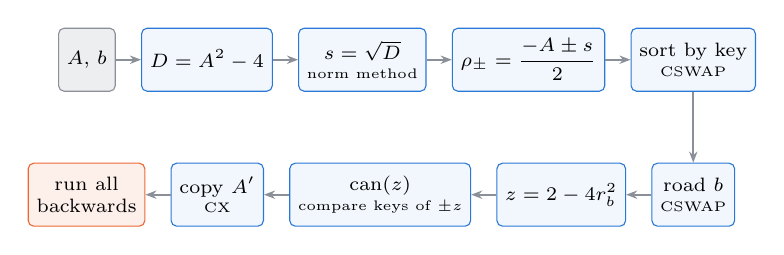
\begin{tikzpicture}[node distance=0.32cm]
\node[box, fill=cgray!15, draw=cgray] (in) {$A$, $b$};
\node[box, right=of in] (d) {$D=A^2-4$};
\node[box, right=of d] (s) {$s=\sqrt D$\\[-1pt]{\tiny norm method}};
\node[box, right=of s] (r) {$\rho_\pm=\dfrac{-A\pm s}{2}$};
\node[box, right=of r] (srt) {sort by key\\[-1pt]{\tiny CSWAP}};
\node[box, below=0.9cm of srt] (rd) {road $b$\\[-1pt]{\tiny CSWAP}};
\node[box, left=of rd] (z) {$z=2-4r_b^2$};
\node[box, left=of z] (sg) {$\can(z)$\\[-1pt]{\tiny compare keys of $\pm z$}};
\node[box, left=of sg] (cp) {copy $A'$\\[-1pt]{\tiny CX}};
\node[box, left=of cp, fill=corange!10, draw=corange] (un) {run all\\backwards};
\foreach \u/\v in {in/d,d/s,s/r,r/srt,srt/rd,rd/z,z/sg,sg/cp,cp/un} \draw[arr] (\u) -- (\v);
\end{tikzpicture}

\vspace{0.6em}
\begin{columns}[T]
\begin{column}{0.48\textwidth}
\begin{block}{Square root from the norm}
\small
$D=\alpha+\beta i$. Two exponentiations in $\mathbb F_p$:
\[ \lambda=(\alpha^2+\beta^2)^{\frac{p+1}4},\ \ \delta=\tfrac{\alpha+\lambda}2,\ \ r=\delta^{\frac{p-3}4}. \]
$y=r\delta$, $t=\beta r/2$, $q=[yr=1]$:\quad
$s=y+ti$ if $q=1$, else $s=-t+yi$.
No inversion (Appendix A5).
\end{block}
\end{column}
\begin{column}{0.48\textwidth}
\begin{itemize}\small
\item No branches: every ``if'' is a flag qubit and controlled gates.
\item Any root $s$ works: the key sort fixes the order of $\rho_\pm$.
\item $|A,b\rangle|0\rangle\mapsto|A,b\rangle|T_b(A)\rangle$, all work qubits back to 0 (Bennett).
\item Clock-Tower test without division: $j\in\mathbb F_p\iff \overline N D=N\overline D$.
\end{itemize}
\end{column}
\end{columns}
\end{frame}

% =========================================================================
\begin{frame}{Part III: building blocks}
\begin{columns}[c]
\begin{column}{0.55\textwidth}
\centering
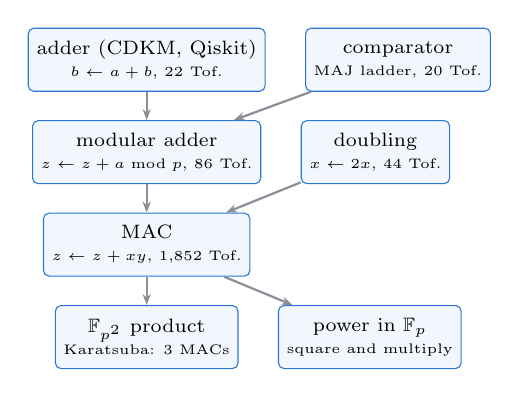
\begin{tikzpicture}[node distance=0.36cm and 0.5cm]
\node[box] (add) {adder (CDKM, Qiskit)\\{\tiny $b\leftarrow a+b$, 22 Tof.}};
\node[box, right=of add] (lt) {comparator\\{\tiny MAJ ladder, 20 Tof.}};
\node[box, below=of add] (ma) {modular adder\\{\tiny $z\leftarrow z+a \bmod p$, 86 Tof.}};
\node[box, right=of ma] (db) {doubling\\{\tiny $x\leftarrow2x$, 44 Tof.}};
\node[box, below=of ma] (mac) {MAC\\{\tiny $z\leftarrow z+xy$, 1{,}852 Tof.}};
\node[box, below=of mac] (m2) {$\mathbb F_{p^2}$ product\\{\tiny Karatsuba: 3 MACs}};
\node[box, right=of m2] (pw) {power in $\mathbb F_p$\\{\tiny square and multiply}};
\draw[arr] (add) -- (ma); \draw[arr] (lt) -- (ma);
\draw[arr] (ma) -- (mac); \draw[arr] (db) -- (mac);
\draw[arr] (mac) -- (m2); \draw[arr] (mac) -- (pw);
\end{tikzpicture}\\[2pt]
{\scriptsize\color{cgray} Toffoli counts for $p=1019$, $n=10$ bits}
\end{column}
\begin{column}{0.43\textwidth}
\begin{itemize}\small
\item Gates: X, CX, Toffoli, CSWAP only.
\item Modular adder: add, subtract $p$, add $p$ back if the sign bit is 1, then clear the flag with the comparator.
\item Doubling is a relabelling of qubits plus one subtraction of $p$.
\item MAC: for each bit $y_i$, add $y_i\cdot x$, then double $x$. This gives $n$ modular adders, so $O(n^2)$.
\item An exponentiation is $O(n)$ products, so one step is $O(n^3)$.
\end{itemize}
\end{column}
\end{columns}
\end{frame}

% =========================================================================
\begin{frame}{Part III: checks at $p=1019$}
\begin{columns}[T]
\begin{column}{0.5\textwidth}
\begin{block}{Every input}
\small
\begin{itemize}
\item Aer matrix-product-state simulator, 587 qubits.
\item Step: 510 inputs (255 spots, both bits). Output $=$ classical $T_b(A)$, inputs unchanged, every work qubit 0. \textbf{510/510.}
\item Clock-Tower test: \textbf{255/255} spots.
\item 32 inputs on random spots at $p=46351$: all correct.
\end{itemize}
\end{block}
\end{column}
\begin{column}{0.46\textwidth}
\begin{block}{Why basis states are enough}
\small
X, CX, Toffoli and CSWAP send basis states to basis states, so the circuit $U$ is a permutation matrix. If $U\ket x\ket0=\ket x\ket{f(x)}$ for every $x$, then by linearity
\[ U\sum_x c_x\ket x\ket0=\sum_x c_x\ket x\ket{f(x)}. \]
\end{block}
\begin{block}{Phases}
\small
64 states $\cos w\ket x+e^{i\phi}\sin w\ket y$ go through the circuit and then the inverse of a reference circuit. All return to $\ket{0}$. A deliberate phase error is detected.
\end{block}
\end{column}
\end{columns}
\end{frame}

% =========================================================================
\begin{frame}{Part III: cost at $p\approx2^{256}$}
\begin{columns}[c]
\begin{column}{0.5\textwidth}
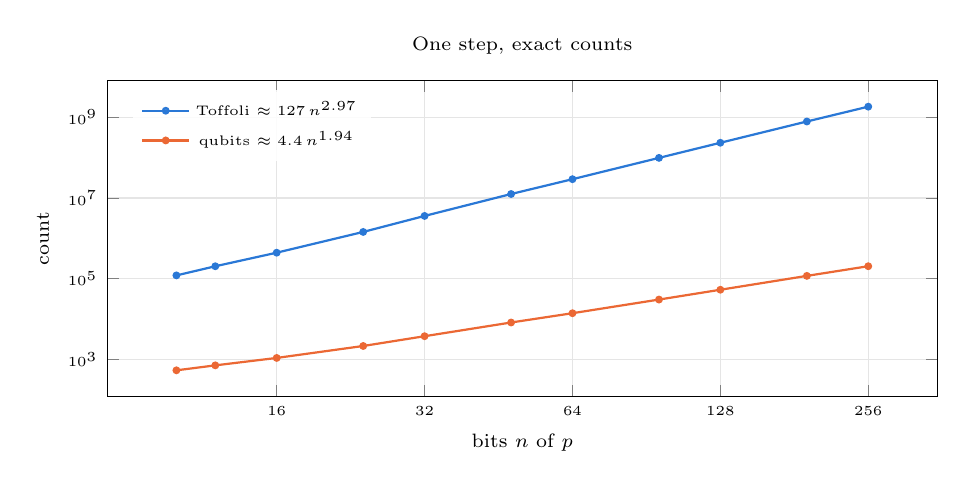
\begin{tikzpicture}
\begin{axis}[width=\linewidth, height=5.6cm, xmode=log, ymode=log, log basis x=2,
  xlabel={bits $n$ of $p$}, ylabel={count}, title={One step, exact counts},
  xtick={16,32,64,128,256}, xticklabels={16,32,64,128,256}, legend pos=north west]
\addplot[cblue, thick, mark=*, mark size=1pt] coordinates {(10,120716) (12,203544) (16,441248) (24,1442192) (32,3592352) (48,12552544) (64,29232784) (96,98595488) (128,233652144) (192,785777392) (256,1833327328)};
\addlegendentry{Toffoli $\approx127\,n^{2.97}$}
\addplot[corange, thick, mark=*, mark size=1pt] coordinates {(10,537) (12,713) (16,1089) (24,2153) (32,3761) (48,8225) (64,13969) (96,30449) (128,53265) (192,117521) (256,204049)};
\addlegendentry{qubits $\approx4.4\,n^{1.94}$}
\end{axis}
\end{tikzpicture}
\end{column}
\begin{column}{0.48\textwidth}
\small
\begin{tabular}{lr}
\toprule
\multicolumn{2}{l}{\textbf{one step}, $n=256$}\\
Toffoli & $1.83\cdot10^9$\\
$T$ (7 per Toffoli) & $1.28\cdot10^{10}$\\
qubits & 204{,}049\\
\midrule
\multicolumn{2}{l}{\textbf{Part II search}, $L=2n=512$}\\
target fraction $q$ & $7/\sqrt p=2^{-124.9}$\\
Grover iterations & $2^{62.1}$\\
Toffoli & $2^{102.9}$\\
two-qubit, $\{cx,rz,sx,x\}$ & $2^{105.9}$\\
depth & $2^{104.4}$\\
logical qubits & 466{,}000\\
\midrule
classical random routes & $2^{133.9}$ steps\\
\bottomrule
\end{tabular}
\end{column}
\end{columns}
\end{frame}

% =========================================================================
\begin{frame}{Part III: trade-offs, other algorithms}
\begin{columns}[c]
\begin{column}{0.5\textwidth}
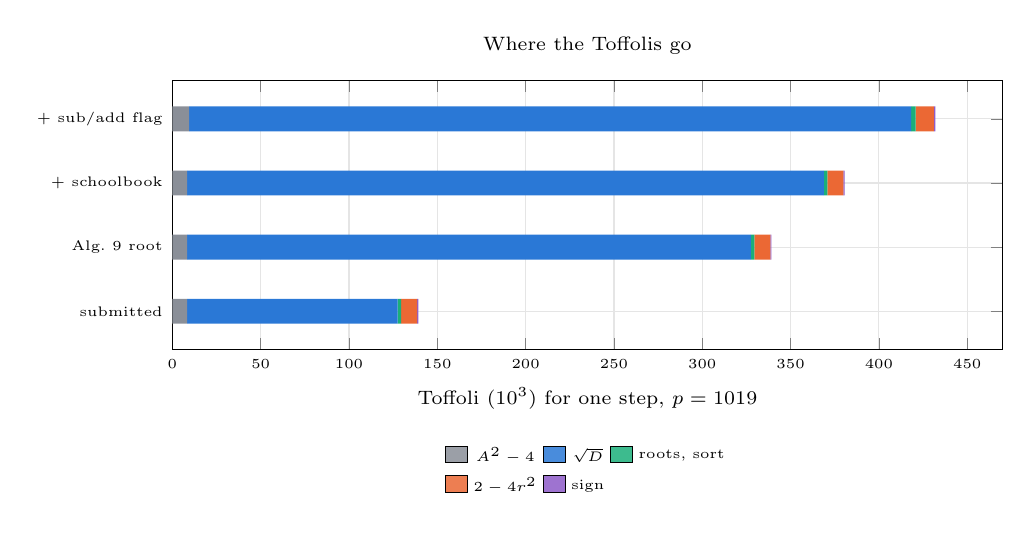
\begin{tikzpicture}
\begin{axis}[width=\linewidth, height=5.0cm, xbar stacked, bar width=9pt,
  xmin=0, xmax=470, xlabel={Toffoli ($10^3$) for one step, $p=1019$}, title={Where the Toffolis go},
  ytick={1,2,3,4}, yticklabels={submitted, Alg.~9 root, + schoolbook, + sub/add flag},
  y tick label style={font=\tiny, align=right},
  ymin=0.4, ymax=4.6, legend columns=3,
  legend style={at={(0.5,-0.32)}, anchor=north}]
\addplot[fill=cgray, draw=none] coordinates {(8.356,1) (8.356,2) (8.356,3) (9.556,4)};
\addlegendentry{$A^2-4$}
\addplot[fill=cblue, draw=none] coordinates {(119.216,1) (319.142,2) (360.486,3) (408.630,4)};
\addlegendentry{$\sqrt{D}$}
\addplot[fill=caqua, draw=none] coordinates {(1.998,1) (1.998,2) (1.998,3) (2.526,4)};
\addlegendentry{roots, sort}
\addplot[fill=corange, draw=none] coordinates {(9.052,1) (9.052,2) (9.052,3) (10.348,4)};
\addlegendentry{$2-4r^2$}
\addplot[fill=cpurple, draw=none] coordinates {(0.614,1) (0.614,2) (0.614,3) (0.854,4)};
\addlegendentry{sign}
\end{axis}
\end{tikzpicture}
\end{column}
\begin{column}{0.48\textwidth}
\small
Each row changes one algorithm of the submitted circuit:

\smallskip
{\scriptsize\setlength{\tabcolsep}{3pt}
\begin{tabular}{lrr}
\toprule
change & Toffoli & factor\\
\midrule
submitted & 139{,}236 & 1.00\\
root: Algorithm 9 ($\mathbb F_{p^2}$ powers) & 339{,}162 & 2.44\\
\ + schoolbook $\mathbb F_{p^2}$ product & 380{,}506 & 2.73\\
\ + flag by subtract and add back & 431{,}914 & 3.10\\
\bottomrule
\end{tabular}}

\smallskip
\begin{itemize}\small
\item The root is 86\% of the step. In $\mathbb F_p$ a product is 1 MAC; in $\mathbb F_{p^2}$ it is 3 or 4.
\item A comparison needs only the carry: $2n$ Toffolis, not $4(n+1)$.
\item At $n=256$: submitted $=0.34\times$ the slowest version.
\end{itemize}
\end{column}
\end{columns}
\end{frame}

% =========================================================================
\begin{frame}{Part III: trade-offs, qubits and depth}
\begin{columns}[c]
\begin{column}{0.5\textwidth}
\begin{block}{Qubits: pebbling}
\small
Bennett keeps each intermediate value: about $1.5n$ registers of $n$ qubits per exponentiation, so qubits $\sim n^2$.

\smallskip
\begin{tabular}{lcc}
\toprule
strategy & registers & steps run\\
\midrule
Bennett (ours) & $T$ & $2T$\\
$\sqrt T$ checkpoints & $2\sqrt T$ & $\approx3T$\\
recursive halving & $\log_2T$ & $T^{1.58}$\\
\bottomrule
\end{tabular}

\smallskip
We keep Bennett: it gives the fewest gates.
\end{block}
\end{column}
\begin{column}{0.48\textwidth}
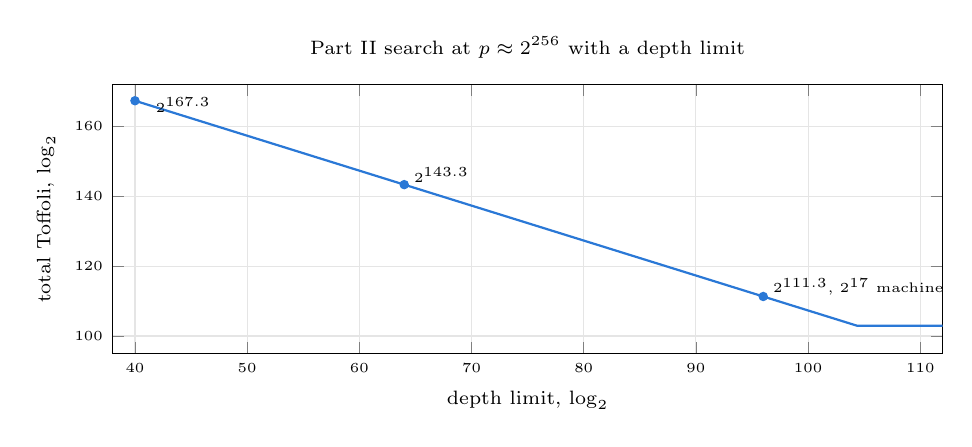
\begin{tikzpicture}
\begin{axis}[width=\linewidth, height=5.0cm, xmin=38, xmax=112, ymin=95, ymax=172,
  xlabel={depth limit, $\log_2$}, ylabel={total Toffoli, $\log_2$},
  title={Part II search at $p\approx2^{256}$ with a depth limit}]
\addplot[cblue, thick] coordinates {(40,167.3) (104.4,102.9) (112,102.9)};
\addplot[cblue, only marks, mark=*, mark size=1.5pt] coordinates {(40,167.3) (64,143.3) (96,111.3)};
\node[font=\tiny, anchor=west] at (axis cs:96,114) {$2^{111.3}$, $2^{17}$ machines};
\node[font=\tiny, anchor=west] at (axis cs:64,146) {$2^{143.3}$};
\node[font=\tiny, anchor=west] at (axis cs:41,166) {$2^{167.3}$};
\end{axis}
\end{tikzpicture}\\
{\scriptsize With depth limit $2^m$: $S=(2^{104.4-m})^2$ machines; total $\times\sqrt S$.}
\end{column}
\end{columns}
\end{frame}

% =========================================================================
\section{Part IV}
\begin{frame}{Part IV: the Djinns}
\begin{columns}[T]
\begin{column}{0.48\textwidth}
\begin{block}{What still works}
\small
\begin{itemize}
\item The graph is the same: degree, roads, cycles, expansion.
\item Classical: random walks ($p^{1/2}$ tower tests), BFS/DFS with a table of names, cycle and collision search.
\item Our Part I method: the survey asks the Djinn for every road ($O(N)$), then the step circuit is built from the survey.
\item With a \emph{coherent} Djinn and volunteer: Grover and quantum walks still give $p^{1/4}$.
\end{itemize}
\end{block}
\end{column}
\begin{column}{0.48\textwidth}
\begin{block}{What stops working}
\small
\begin{itemize}
\item Arithmetic on $A$: the Part III step circuit, the $j$ test, Frobenius.
\item Methods from number theory (class groups, endomorphism rings).
\item A human Djinn or volunteer answers one question at a time. No superposition, so no Grover.
\end{itemize}
\end{block}
\begin{block}{Lower bound}
\small
The names are random, so the volunteer is close to a black box. The $\Omega(p^{1/4})$ bound needs one more condition: the tower set must not be visible from the graph shape.
\end{block}
\end{column}
\end{columns}
\end{frame}

% =========================================================================
\begin{frame}{Summary}
\begin{columns}[T]
\begin{column}{0.55\textwidth}
\begin{itemize}\small
\item \textbf{Part I:} all 37 passwords, $k$ counted at confidence $\ge0.99$, survey rules kept.
\item \textbf{Part II:} $p^{1/4+o(1)}$ quantum against $p^{1/2+o(1)}$ classical. Black-box lower bound; a lower bound for the real arithmetic would prove P $\ne$ NP. Fitted exponent $0.523\pm0.040$; Grover demo $=$ theory.
\item \textbf{Part III:} one step from arithmetic only, 510/510 correct. At $2^{256}$: $1.8\cdot10^9$ Toffolis per step, $2^{103}$ for the search.
\item \textbf{Part IV:} the speed-up needs coherent access, not the names.
\end{itemize}
\end{column}
\begin{column}{0.42\textwidth}
\begin{block}{Reproduce}
\scriptsize
\texttt{uv run oasis --part 1 --p 1019 \char`\\}\\
\texttt{\ \ --A0 "977 + 297i" --L 12 \char`\\}\\
\texttt{\ \ --jstar "797 + 921i"}\\
\texttt{uv run oasis --part 2}\\
\texttt{uv run oasis --part 3}\\[3pt]
Results: \texttt{results/}
\end{block}
\end{column}
\end{columns}
\end{frame}

% =========================================================================
\appendix
\begin{frame}{A1. Iterative Amplitude Estimation}
\small
\begin{itemize}
\item Problem: $A\ket0=\sqrt{a}\ket{\text{good}}+\sqrt{1-a}\ket{\text{bad}}$. Estimate $a=\sin^2\theta_a$.
\item Grover operator $Q=A S_0 A^\dagger S_{\rm good}$. Then $Q^mA\ket0$ is good with probability $\sin^2((2m+1)\theta_a)$.
\item Each round picks the largest power $m$ that keeps $(2m+1)\theta_a$ inside one half-period of the current interval. It measures, and narrows the interval for $\theta_a$ (Clopper--Pearson).
\item Cost: $O\!\left(\frac1\varepsilon\log\frac{2}{\alpha}\log\frac{\pi}{4\varepsilon}\right)$ queries for error $\varepsilon$ at confidence $1-\alpha$, with no QFT (Grinko, Gacon, Zoufal, Woerner 2021).
\item Here: good $=$ spot register at an ANC code, $a=k/N$. We halve $\varepsilon$ until the interval for $k=aN$ holds one integer; $\alpha=0.01$.
\end{itemize}
\end{frame}

\begin{frame}{A2. Theorems we use}
\small
\begin{description}[Lubetzky--Peres]
\item[Deuring--Eichler] For $p\equiv3\pmod4$, the number of supersingular $j\in\mathbb F_p$ is $2h(-p)$ if $p\equiv3\pmod8$ and $h(-p)$ if $p\equiv7\pmod8$.
\item[Siegel] $h(-p)=p^{1/2+o(1)}$.
\item[Pizer] The supersingular 2-isogeny graph is 3-regular and Ramanujan: every nontrivial eigenvalue has $|\lambda|\le2\sqrt2$.
\item[Lubetzky--Peres] For a walk without backtracking of length $L$ on a $3$-regular Ramanujan graph with $N_E$ directed edges: $\big\|\tilde\mu_L/\pi_E-1\big\|^2_{L^2}\le2N_E2^{-L}(8L^2+1)$.
\item[BBBV, Zalka] Search for one of $k$ marked items among $N$ with a black-box oracle needs $\Omega(\sqrt{N/k})$ queries; Grover is optimal.
\item[BBHT] With $k$ unknown and $\lambda=6/5$, the expected number of Grover iterations is at most $\tfrac94\sqrt{N/k}$.
\end{description}
\end{frame}

\begin{frame}{A3. The Clock-Tower problem is in NP}
\small
Decision problem: given $p$ and $A_0$, is there a route of length $L=O(\log p)$ that ends on the Clock Tower?
\begin{enumerate}
\item \textbf{Certificate:} the route $x=b_1\cdots b_L$. Its length is $O(\log p)$ bits.
\item \textbf{Check:} $L$ steps, each a fixed number of operations in $\mathbb F_{p^2}$ (one square root is one exponentiation), then compute $j$ and test $\operatorname{Im} j=0$. Each operation costs $\mathrm{poly}(\log p)$, so the check costs $\mathrm{poly}(\log p)$.
\item So the problem is in NP. The input size is $n=\log_2p$.
\item Our cost $p^{1/4}=2^{n/4}$ is exponential in $n$. A proof that no polynomial-time quantum algorithm exists would show NP $\not\subseteq$ BQP. Since P $\subseteq$ BQP, this gives P $\neq$ NP.
\item So an unconditional lower bound for the real arithmetic is out of reach today. Lower bounds exist only in a model with a black-box oracle.
\end{enumerate}
\end{frame}

\begin{frame}{A4. Known algorithms that use the arithmetic}
\small
\begin{tabular}{L{3.0cm}L{3.0cm}L{1.7cm}L{4.3cm}}
\toprule
algorithm & solves & cost & why not here\\
\midrule
Biasse--Jao--Sankar (2014) & path between two curves, quantum & $\widetilde O(p^{1/4})$ & same exponent as Grover\\
Page--Wesolowski (2023) & path, classical, from both ends & $\widetilde O(p^{1/2})$ & meet-in-the-middle; forbidden by the rules\\
Delgado (2026) & one endomorphism, classical & $p^{1/3+o(1)}$ & not a fixed-degree path; the path version needs GRH and gives longer paths\\
Wesolowski (2021) & path $\Leftrightarrow$ endomorphism ring & reduction & assumes GRH\\
\bottomrule
\end{tabular}

\medskip
None of these gives less than $p^{1/4}$ for a route of length $\Theta(\log p)$ from $A_0$ under the rules.
\end{frame}

\begin{frame}{A5. Proof of the square root from the norm}
\small
Let $s=x_0+x_1i$ with $s^2=D=\alpha+\beta i$. Then $x_0^2-x_1^2=\alpha$, $2x_0x_1=\beta$, and $(x_0^2+x_1^2)^2=\alpha^2+\beta^2=m$.
\begin{itemize}
\item $m$ is a square in $\mathbb F_p$, so $\lambda=m^{(p+1)/4}$ gives $\lambda^2=m$, and $x_0^2+x_1^2=\pm\lambda$.
\item $\delta=(\alpha+\lambda)/2$ and $\delta'=(\alpha-\lambda)/2$ satisfy $\delta\delta'=-\beta^2/4$. Since $-1$ is not a square ($p\equiv3\bmod4$), exactly one of them is a square (if $\beta\ne0$).
\item $r=\delta^{(p-3)/4}$, $y=r\delta$: then $y^2=\delta^{(p+1)/2}=\pm\delta$ and $yr=\delta^{(p-1)/2}=\pm1=q$-flag.
\item $q=1$: $y^2=\delta=x_0^2$, $x_1=\beta/(2y)=\beta r/2=t$, so $s=y+ti$.
\item $q=0$: $y^2=-\delta=x_1^2$, $x_0=\beta/(2y)=-\beta r/2=-t$, so $s=-t+yi$.
\item $\delta=0$ only if $\beta=0$ and $\alpha$ is not a square; then $\delta:=\alpha$ gives $q=0$, $s=yi$ with $y^2=-\alpha$.
\end{itemize}
Checked on every nonzero square for 13 primes $\le83$, and in the circuit on random squares at $p=43$ and $p=131$.
\end{frame}

\begin{frame}{A6. Resources}
\scriptsize
\begin{columns}[T]
\begin{column}{0.48\textwidth}
\textbf{Part I}, $p=1019$, $L=12$, $\{cx,rz,sx,x\}$, level 1\\[2pt]
\begin{tabular}{lrrr}
\toprule
 & queries & CX & depth\\
\midrule
one step & 1 & 13{,}395 & 42{,}173\\
Grover iteration & 24 & 319{,}106 & 1{,}009{,}282\\
\bottomrule
\end{tabular}\\
22 qubits. Total: 854{,}784 queries to count, 26{,}304 to search.

\medskip
\textbf{Part II}, $p=5923$, $L=12$, $\{cx,rz,sx,x\}$, level 1\\[2pt]
\begin{tabular}{lrrr}
\toprule
 & queries & CX & depth\\
\midrule
one step & 1 & 141{,}813 & 462{,}568\\
Grover iteration & 24 & 3{,}401{,}466 & 11{,}100{,}684\\
search, $t=4$ & 96 & 13{,}605{,}864 & 44{,}402{,}739\\
\bottomrule
\end{tabular}\\
25 qubits.
\end{column}
\begin{column}{0.5\textwidth}
\textbf{Part III}, $p=1019$, $\{x,cx,ccx\}$; two-qubit in $\{cx,rz,sx,x\}$ $=$ CX $+6\cdot$Toffoli\\[2pt]
\begin{tabular}{lrrrr}
\toprule
 & qubits & Toffoli & 2-qubit & depth\\
\midrule
step & 587 & 139{,}236 & 1{,}127{,}164 & 307{,}933\\
tower test & 192 & 37{,}794 & -- & 63{,}148\\
\bottomrule
\end{tabular}\\
$T$: 974{,}652 (7 per Toffoli) or 556{,}944 (4 per Toffoli).

\medskip
\textbf{Part III}, $n=256$\\[2pt]
\begin{tabular}{lr}
\toprule
step: Toffoli / qubits & $1.83\cdot10^9$ / 204{,}049\\
tower test: Toffoli & $2.1\cdot10^7$\\
search: Toffoli / depth & $2^{102.9}$ / $2^{104.4}$\\
\bottomrule
\end{tabular}
\end{column}
\end{columns}
\end{frame}

\begin{frame}{A7. Note on the phase test}
\small
\begin{itemize}
\item The test prepares $\cos w\ket{0}\ket x+e^{i\phi}\sin w\ket1\ket y$, runs the new circuit, then the inverse of the reference circuit, then undoes the preparation. The result is $\ket0$ with probability $1-\sin^2(2w)\sin^2(\Delta\theta/2)$.
\item A path of pairs through the inputs gives $\theta(x)=\theta(y)$ for all of them: the two circuits are equal up to one global phase.
\item With equal amplitudes ($w=\pi/4$), Aer's matrix-product-state simulator lost the relative phase for some values of $\phi$, also for a circuit followed by its own inverse. Two equal Schmidt values make the SVD degenerate.
\item With $w=0.55$ every case passes. A deliberate error ($Z$ on $b$) is found on every pair with different $b$, and only there.
\end{itemize}
\end{frame}

\end{document}
